\documentclass{ximera}
\usepackage{sagetex}
%% handout
%% space
%% newpage
%% numbers
%% nooutcomes
 
%% You can put user macros here
%% However, you cannot make new environments

\graphicspath{{./}{module1Activity/}{module2Activity/}{module3Activity/}}

\usepackage{sagetex}
\usepackage{tikz}
\usepackage{hyperref}
\usepackage{tkz-euclide}
\usetkzobj{all}
\pgfplotsset{compat=1.7} % prevents compile error.

\tikzstyle geometryDiagrams=[ultra thick,color=blue!50!black]
 %% we can turn off input when making a master document
 
\outcome{}
\author{Darryl Chamberlain Jr.}
  
\title{Objective 2 - Identify Exponential Model}
 
\begin{document}
\begin{abstract}

\end{abstract}

\maketitle
 
% Link to textbook
Link to textbook: 
\href{https://cnx.org/contents/mwjClAV_@8.21:_tqWoaDz@17/Exponential-and-Logarithmic-Models}{Identify when a real-world situation would require an exponential model.}

\textbf{Note: There is currently no video for this objective. This activity is built as an ``interactive activity", akin to what you would expect in a live lecture.}
 
%%%%%%%%%%%%%%%%%%%%%
%%%  Objective 2  %%%
%%%%%%%%%%%%%%%%%%%%%

\begin{center} \textbf{\Large Introduction} \end{center}

Now that we have looked at logarithmic models, we can look at their natural counter-part: exponential models. 

\begin{theorem}
	\textbf{Need for an Exponential Model}
	
	A exponential model is appropriate when the quantities change slowly at first, then rapidly \textbf{later on}. 
	
	\begin{figure}
		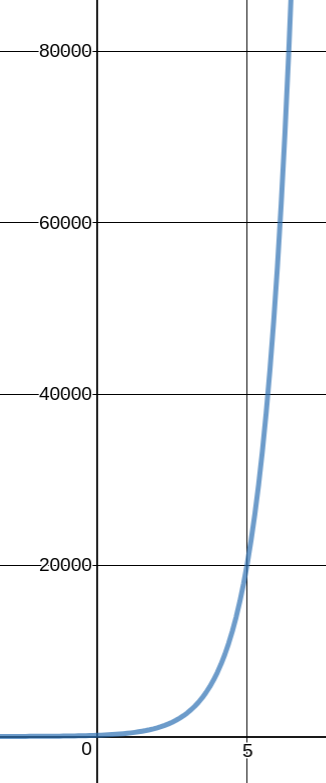
\includegraphics[scale=0.3]{expGrowth.png}
		\caption{Exponential growth, characterized by a slow growth early, then a rapid growth later on.}
	\end{figure}
	
	\begin{figure}
		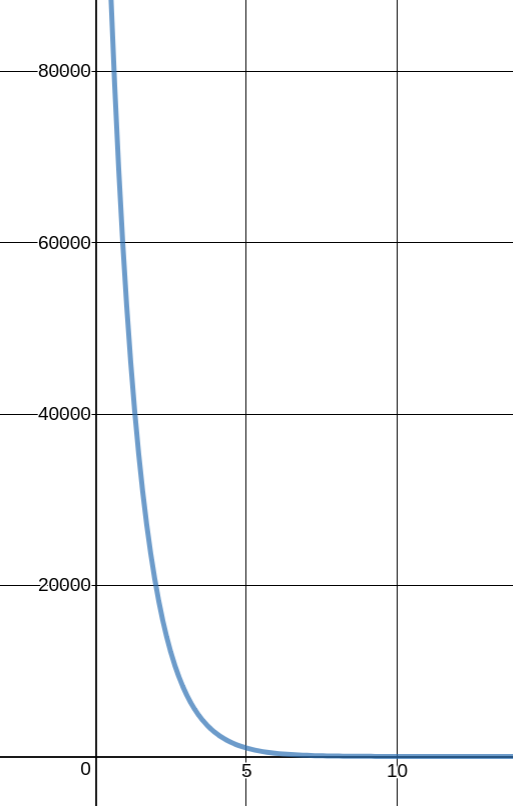
\includegraphics[scale=0.3]{expDecay.png}
		\caption{Exponential decay, characterized by rapid decay initially, then a slow decay later.}
	\end{figure}
	
\end{theorem}

We saw this issue before: \textbf{it is extremely difficult to distinguish between $e^{-x}$ and $-\log(x)$ just based on rates of change}! Let's look closer at two examples below:

\begin{figure}
	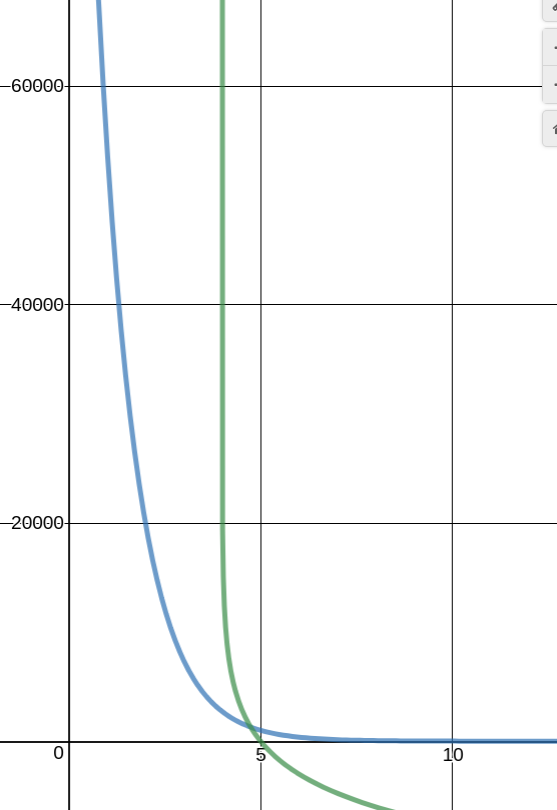
\includegraphics[scale=0.3]{comparison.png}
	\caption{Comparing $ae^{-x}$ (blue) and $-a\log(x)$ (green).}
\end{figure}

\begin{question}
	Use the words ``bounded" and ``unbounded" to describe the difference between these two functions.
	
	We know the blue line is an exponential function because it is $\answer[format=string]{bounded}$ near $y=0$ and we know the green line is a logarithmic function because it is $\answer[format=string]{unbounded}$ near $y=0$. 
\end{question}

\begin{center} \textbf{\Large Common Exponential Models} \end{center}

\begin{itemize}
	\item \textbf{Bacterial (unbounded) growth:} $P = P_0e^{rt}$, where $P_0$ is the initial bacteria population, $r$ is the rate the bacteria multiply, and $t$ is time. 
	\item \textbf{Population (bounded) growth:} $P = \frac{c}{1+ae^{-bx}}$, where $c$ is the carrying capacity, $\frac{c}{1+a}$ is the initial population, and $b$ is the rate of growth.  
	\item \textbf{Continuously compounded interest:} $A = Pe^{rt}$, where $P$ is the principle (initial money), $r$ is the rate of interest, and $t$ is time.
	\item \textbf{Newton's Law of Cooling:} $T(t) = ae^{kt} + T_s$, where $t$ is time, $A$ is the difference between initial temperature of object and surroundings, and $k$ is the continuous rate of cooling of the object. This model would be used to determine how long a body has been deceased for.
	\item \textbf{SIS Model:} This describes the infection of a population when the infection does \textbf{not} provide any resistance after infection. Rather than provide an explicit equation, \href{http://rocs.hu-berlin.de/D3/herd/}{check out this dynamic figure (keep vaccination at 0 to see what an SIS model looks like).} 
\end{itemize}

\begin{center} \textbf{\Large Identifying Exponential Models} \end{center}

\begin{question}
	Your bank offers a savings account that will increase your total balance by 0.2\% annually. You want to decide how much to initially deposit and if the initial deposit makes a big difference in the long run. Should we model this scenario using an exponential function?
	
	$\answer[format=string]{Yes}$
	
	\begin{feedback}
		Compound interest can be modeled by $P = A (1 + \frac{r}{n})^{nt}$, were $P$ is the principle (initial money), $r$ is the rate of interest, $t$ is time, and $n$ is the number of times it compounds per time unit in $t$. Even though the base is not $e$, this is still an exponential function!
	\end{feedback}
\end{question}

\begin{question}
	A population of bacteria doubles every hour. Should we model the scenario with an exponential function?
	
	$\answer[format=string]{Yes}$
	
	\begin{feedback}
		Our two quantities are population $P$ and time $t$ (in hours). If we want it to double every hour, we want to multiply by 2 every time $t$ increases - we would write that as $2^t$. Combining that with the initial population $P_0$, we would get the equation $P(t) = P_0 2^t$. Again, exponential functions are more than just $e^x$ - they are any number raised to your variable.
	\end{feedback}
\end{question}

\begin{question}

\begin{figure}
	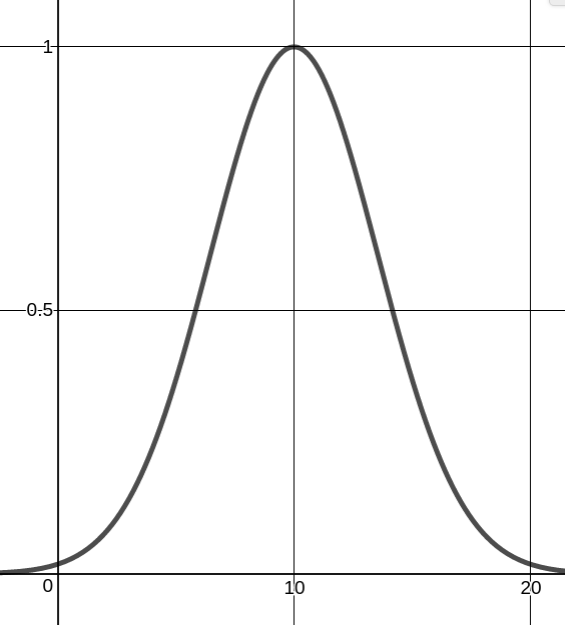
\includegraphics[scale=0.3]{expSquared.png}
	\caption{Normal distribution curve.}
\end{figure}

Should we model the normal distribution curve above by an exponential function?

$\answer[format=string]{Yes}$

\begin{feedback}
Here is an example of why are heuristics are too simple: log and exponential functions can have polynomials as variables rather than just $x$. The picture above is a translated version of $e^{-x^2}$. We can see the ``exponential" patterns as we approach 10 and as we move away from 10. You would not be expected to have realized this on the exam, but this is just to show that exponential and logarithmic functions can look very different from the elementary version $a^x$ and $\log(x)$.
\end{feedback}

\end{question}

\end{document}